\documentclass[conference]{IEEEtran}

\usepackage{cite}
\usepackage{amsmath,amssymb,amsfonts}
\usepackage{algorithmic}
\usepackage{graphicx}
\usepackage{textcomp}
\usepackage{xcolor}


\usepackage{times}
\usepackage[mediumspace,mediumqspace,Gray,squaren]{SIunits}
\usepackage[cmex10]{amsmath}
%Use for Hightlighting

% This is for Sub-figures
\usepackage[hang,center,tight]{subfigure}
\usepackage{float}
\usepackage{graphicx}

% This is for Graphic
%\usepackage[pdftex]{graphicx}

% This is for citation
\usepackage[hyphens,obeyspaces]{url}
\usepackage{cite}
\usepackage[none]{hyphenat}
%\usepackage{caption}
\tolerance=9999
\emergencystretch=10pt
\hyphenpenalty=10000
\exhyphenpenalty=100

\usepackage{booktabs}
\usepackage{textgreek}

% This is for Table Package
%\usepackage{tabu}
\usepackage{booktabs}
\usepackage{threeparttable}
\usepackage{multirow}

% Hyper Extension
%\usepackage[none]{hyphenat}

% LaTeX the ability to create hyperlinks within the document
%\usepackage[colorlinks=false,hidelinks]{hyperref}

% for any plug-in code... insert it here. For example, the CDC style...
%\usepackage{ieeecdc}

%\usepackage{ifthen}
%\newboolean{includefigs}
%\setboolean{includefigs}{false}
%\newcommand{\condcomment}[2]{ifthenelse{#1}{#2}{}}
%\input{endpics} % endpics.tex includes all the figures and tables

% This is for Algorithm Writing
\usepackage{algorithm}
\usepackage{algorithmic}
% \usepackage{algpseudocode}
\renewcommand{\algorithmicrequire}{\textbf{Input:}}
\renewcommand{\algorithmicensure}{\textbf{Output:}}
\renewcommand{\algorithmiccomment}[1]{/* #1 */}

\newtheorem{definition}{\textbf{Definition}}
\newtheorem{problem}{\textbf{Problem}}
\newcommand{\prob}[2]{\begin{problem}[#1] #2 \end{problem}}
\newtheorem{scenario}{\textbf{Scenario}}
\newcommand{\scen}[2]{\begin{scenario}[#1] #2 \end{scenario}}

\usepackage{textcomp} % \textmu \textohm
%\usepackage{fixltx2e} % \textsuperscript

%\ This is for comment
\usepackage{verbatim}

\usepackage{lineno}
%\linenumbers

\usepackage [english]{babel}
\usepackage{blindtext}
\pagestyle{empty}

%\newcommand{\upcite}[1]{\textsuperscript{\textsuperscript{\cite{#1}}}}
\begin{document}
\bstctlcite{IEEEexample:BSTcontrol}
\graphicspath{{./figures/}{./biography/}{./}}

%----------------------------------------------------------------------
% Title Information, Abstract and Keywords
%-----------------------------------------------
\title{SpiceModelIR: Cross-Simulator SPICE Translation via Semantic IR and Intelligent Parameter Inference}

% rmb to comment this for apccas submission
% \author{
% Shen Ni Lee$^{1,2}$,
% Haochen Du$^{1}$,
% Kian Kit Cheah$^{1,2}$,
% Chao Wang$^{1}$,
% Kainlu Low$^{1}$, \\
% Harikrishnan Ramiah$^{2,}$*, and
% Yongfu Li$^{1,3,}$* \\
% 1. School of Integrated Circuits, Shanghai Jiao Tong University, Shanghai, China. \\
% 2. Department of Electrical Engineering, University of Malaya, Malaysia. \\
% \thanks{
% This work is supported in part by the National Natural Science Foundation of China under Grants No. 62350610271 and 62201340, and in part by the Explorers Program of Shanghai (Basic Research Funding) under Grant No. 24TS140020.
% The corresponding authors are 
% Harikrishnan Ramiah (hrkhari@um.edu.my), and
% Yongfu Li (yongfu.li@sjtu.edu.cn).}
% }

\maketitle

\begin{abstract}
SPICE portability still breaks across Cadence Spectre, Synopsys HSPICE, and Berkeley ngspice because production PDKs encode different syntax, expression rules, corner-file dependencies, and BSIM limits. Manual translation is slow and brittle. SpiceModelIR addresses this with a physics-aware intermediate representation, parameter inference for missing process symbols, and closed-loop verification that separates true translation defects from simulator guardrails. Evaluated on 15 PDKs, the system translated 6,638 models and passed all 587 verification tests.
\end{abstract}

\begin{IEEEkeywords}
SPICE simulation, model translation, format conversion, parameter mapping, closed-loop validation, semiconductor design automation, intermediate representation.
\end{IEEEkeywords}

\section{Introduction}
\label{sec:introduction}

\IEEEPARstart{W}{hile} SPICE simulation is used extensively in semiconductor design \cite{Pratap_2014, Kundert_1995, Vogt_ngspice, a2024_single}, translation across Spectre, HSPICE, and ngspice still breaks on syntax, corner dependencies, and BSIM constraints \cite{Chhabria_2025, Goldman_2000}. Teams waste hundreds of engineer-hours on manual rewrites that preserve text but lose device meaning \cite{Dahad_2021, spiceerror, engineererror, a2024_kb}. Existing structural parsers help for Verilog-A bridging, but they do not solve transistor-level portability \cite{Shao_2023_V2Va, Wang_2024_V2VaPlus}.

A second barrier is missing process-dependent parameters. PDKs often separate transistor models from corner-definition files, so variables like \texttt{tox\_default} or \texttt{u0\_n} disappear during translation and break simulation \cite{Hu_1996}. If a tool zero-initializes these symbols, oxide thickness or mobility becomes non-physical and the DC solve fails. LLM-based helpers now support datasheet extraction and netlist curation \cite{Chen_2025_D2S, Chen_2024_DocEDA, Bhandari_2024, Vungarala_2024_SPICEPilot}, but they still do not recover the semantics needed for cross-dialect translation. Generic netlist rewriters \cite{DallOra_2025} also miss the physics constraints, so manual porting remains the default \cite{Zhu_2012, spicesec2025}.

To address these limitations, this paper introduces SpiceModelIR, a semantic pipeline grounded in device physics \cite{Vladimirescu_1994, Tuinenga_1995, Tsividis_2011, Sze_2007, Baker_2010, Rabaey_2003, Lee_2004, Mead_1980, Cheng_1999_MOSFET, Chauhan_BSIMCMG_2020}. SpiceModelIR combines a physics-aware intermediate representation (IR), an inference engine for missing process symbols, and automated verification that filters simulator-side guardrails. Across 15 PDKs, the system passes 587 of 587 verification tests.
%==============================================================================
\section{Intermediate Representation Design}
\label{sec:ir_design}
%==============================================================================
\vspace{-0.6cm}
\subsection{Problem taxonomy and workflow mapping}
Table~\ref{tab:critical_diffs} defines the critical problems P1--P6 that the workflow must resolve. Figure~\ref{fig:master_architecture} should label these problems inside the workflow so the reader can see which phase fixes which failure.

\begin{table*}[!t]
\caption{Top translation problems across SPICE dialects (P1--P6). The workflow figure resolves these problems, so the table intentionally lists only the problem categories and concrete dialect examples.}
\label{tab:critical_diffs}
\centering
\footnotesize
\begin{tabular}{@{}p{1.5cm}p{4.5cm}p{4.7cm}p{4.5cm}@{}}
\toprule
\textbf{Problem ID} & \textbf{Critical issue} & \textbf{HSPICE / Spectre example} & \textbf{ngspice impact} \\
\midrule
P1 & Missing corner symbols & \texttt{tox=\{tox\_def\}}, \texttt{u0=\{u0\_eff\}}, absent \texttt{.include} corner file & Unresolved symbol or zero-initialized parameter breaks DC solve \\
P2 & BSIM level mismatch & HSPICE BSIM4 uses \texttt{level=54}; Spectre uses model keywords rather than the same numeric level & Copying the source level directly causes rejection \\
P3 & Spectre-only expressions & Ternary logic, nested functions, and operator precedence in Spectre expressions & Parser fails or emits invalid algebra \\
P4 & Hierarchy and include structure & \texttt{.lib/.endl}, sections, and nested wrapper files & Relative paths break after porting \\
P5 & Scaling vs. delta parameters & \texttt{u0\_eff} multiplies nominal mobility; \texttt{delvto} shifts threshold voltage & Zeroing the wrong term destroys physical behavior \\
P6 & Simulator guardrails & Valid syntax but invalid geometry, such as BSIM4 envelope violations & ngspice rejects the deck even after translation \\
\bottomrule
\end{tabular}
\end{table*}

\subsection{Semantic IR structure}
The semantic IR stores each device as a typed record, not as a flat text line. The parser first builds an AST. The semantic layer then converts that AST into a compact IR that preserves device type, BSIM family, parameters, units, and dependency edges. Algebraic expressions are stored as trees. When the same symbolic subexpression appears more than once, the implementation may reuse a DAG node internally. The emitted netlist still follows the tree form so the result remains readable.

\paragraph{IR data structure.}
The canonical IR is a device-centric record with explicit fields for syntax, physics, and dependencies.

\begin{center}
\footnotesize
\begin{minipage}{0.97\columnwidth}
\ttfamily
DeviceIR ::= \{ name, kind, bsim, level, params, constraints, includes, provenance \}\newline
ParamNode ::= \{ key, value, unit, status \}\newline
ExprNode ::= Const | Symbol | Unary | Binary | Ternary
\end{minipage}
\end{center}

The IR stores algebraic expressions as trees. When the same symbolic subexpression appears more than once, the implementation may reuse a DAG node internally. Emission back to text still follows the tree form so the result remains readable.

\begin{figure}[!t]
\centering
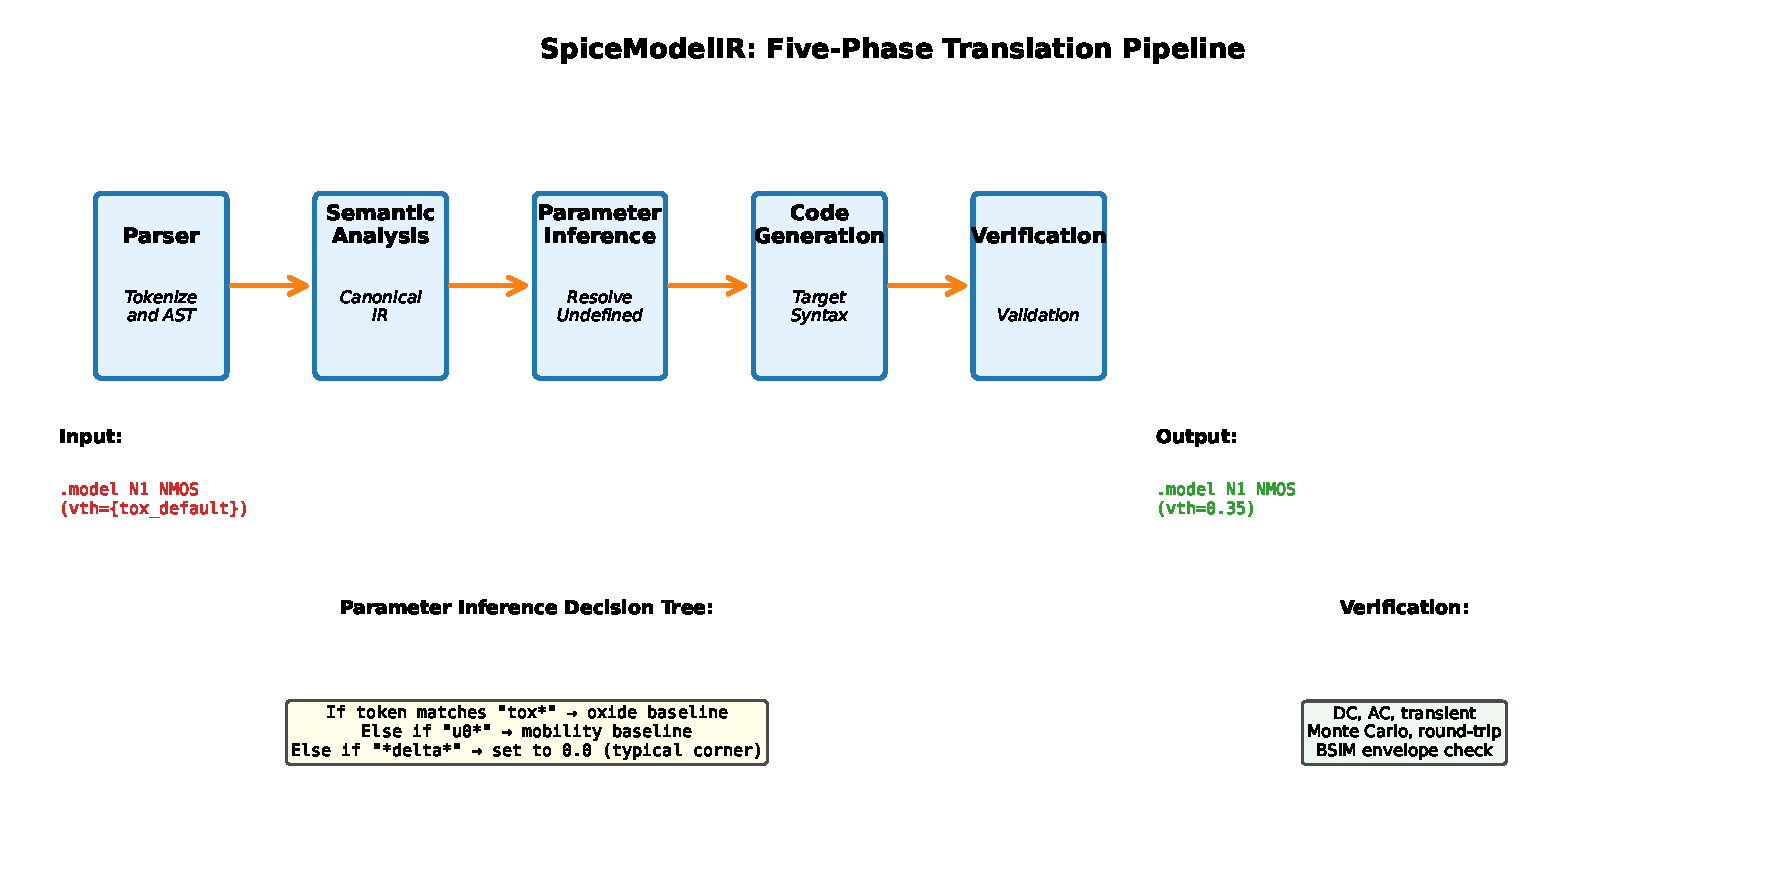
\includegraphics[width=\columnwidth]{fig_architecture.pdf}
\caption{Workflow diagram. Problem labels P1 to P6 are taken from Table~\ref{tab:critical_diffs}. The parsing, IR, inference, and verification stages each resolve a subset of those problems.}
\label{fig:master_architecture}
\end{figure}

\subsection{IR example}
For example, the source line below contains nested ternary logic and a BSIM-related threshold expression.

\begin{center}
\footnotesize
\begin{minipage}{0.97\columnwidth}
\ttfamily
.model MN1 NMOS level=54\newline
    vth0=(t==1 ? vth\_base + dvth0\_corner : vth\_base)\newline
    u0=u0\_core*u0\_eff\newline
    tox=tox\_default
\end{minipage}
\end{center}

In the AST, the expression is split into a conditional node, two additive branches, and one multiplicative node. In the IR, the same record becomes:

\begin{center}
\footnotesize
\begin{minipage}{0.97\columnwidth}
\ttfamily
device: NMOS\newline
bsim: BSIM4\newline
level: 54 -> 14\newline
params:\newline
    vth0 = if(t==1, vth\_base + dvth0\_corner, vth\_base)\newline
    u0   = u0\_core * u0\_eff\newline
    tox  = unresolved(tox\_default)\newline
dependencies:\newline
    dvth0\_corner -> corner file\newline
    u0\_eff -> scaling factor
\end{minipage}
\end{center}

The path from source text to target text is HSPICE text $\rightarrow$ parser AST $\rightarrow$ semantic IR $\rightarrow$ ngspice text. In the parser AST, the ternary is still syntax-specific. In the semantic IR, the branch conditions and parameter roles are explicit. In the emitted ngspice deck, the same device is written with target-compatible syntax and resolved values.

\vspace{-0.6cm}

\section{Translation and Inference Algorithms}
\label{sec:algorithms}
\vspace{-0.6cm}
\subsection{Mapping rules}
Semantic analysis is not a token swap. It performs three kinds of mapping. First, it rewrites cross-dialect expressions into a shared algebraic form, so Spectre ternaries and nested functions can be emitted in a simpler target-safe structure. Second, it resolves hierarchical names such as \texttt{xA.xB.z} by converting simulator-specific separators into a canonical scope path. Third, it separates scaling factors from delta parameters with symbol-level rules: terms ending in \texttt{_eff} or \texttt{_scale} multiply nominal values, while terms beginning with \texttt{del} or \texttt{d} shift them additively. Context-free syntax is handled by the parser, but context-sensitive rewrites use device type, BSIM family, and parameter role. That is why \texttt{pwr(\cdot)} becomes \texttt{pow(\cdot)} during lowering, while \texttt{xA.xB.z} is rewritten using hierarchy metadata rather than a blind string replace.

\subsection{Algorithm 1: Physics-aware parameter inference}
\begin{algorithm}[!t]
\caption{Physics-Aware Parameter Inference}
\label{alg:inference}
\begin{algorithmic}[1]
\REQUIRE IR parameter list $P$, source corpus $C$, rule base $R$
\ENSURE Resolved parameters $P'$
\FOR{each parameter $p \in P$}
    \IF{$p$ is already numeric}
        \STATE keep $p$
    \ELSIF{$p$ matches a delta pattern such as \texttt{del*}}
        \STATE assign $0.0$
    \ELSIF{$p$ matches a scaling pattern such as \texttt{*_eff} or \texttt{*_scale}}
        \STATE assign $1.0$
    \ELSIF{$p$ matches a physics pattern such as \texttt{tox*}, \texttt{u0*}, or \texttt{vth*}}
        \STATE query $R$ for baseline value
        \IF{baseline missing}
            \STATE compute corpus statistic from $C$ using local-family median
        \ENDIF
        \STATE assign baseline
    \ELSE
        \STATE keep as unresolved and mark for verification
    \ENDIF
\ENDFOR
\STATE return $P'$
\end{algorithmic}
\end{algorithm}

The priority order is explicit: numeric values first, delta terms second, scaling terms third, physics-specific tokens fourth, and unresolved values last. Corpus scanning is local and conservative. It reads the same PDK family first, then nearby model files in the same technology node, and uses the median rather than the mean when several files expose the same physical parameter. That keeps one outlier from distorting the inferred baseline. If a local family has no usable sample, the rule base supplies a fixed physics baseline.

\vspace{-0.6cm}

\section{Closed-loop Verification System}
\label{sec:verification}
\vspace{-0.6cm}
\subsection{Filter mechanism}
The constraint-aware filter reads simulator log files and classifies each failure line against a rule base. If the log matches a known backend limit, the run is recorded as a guarded rejection rather than a translation bug. The filter therefore works on simulator stderr/stdout logs after each test bench run, parses the failure string, and matches it against known patterns. For example, one rule marks ngspice BSIM geometry-envelope failures as expected when the generated model is still physically valid.

\begin{itemize}
    \item Rule 23: if the log contains a BSIM geometry-envelope message and the model matches a known BSIM4 family, mark it as simulator-side.
    \item Rule 41: if the log reports a missing symbol after translation, mark it as a translator defect.
    \item Rule 52: if the log reports a geometry-limit error and the offending dimension is below the documented simulator minimum, keep the translation and suppress the failure from the pass-rate count.
\end{itemize}

The filter therefore does not hide failures. It separates backend limitations from real translation defects so the reported pass rate reflects the quality of the translation pipeline.


%----------------------------------------------------------------------
\section{Experimental Results}
\label{section:results}
%----------------------------------------------------------------------
\subsection{Pipeline Validation and Error Resolution Analysis}
\label{sec:results-ablation}
To rigorously validate that the four-stage pipeline is necessary rather than over-engineered, we conducted a controlled ablation experiment. By progressively enabling each phase, we measured the incremental contribution to the overall pass rate as visualized in Table \ref{tab:ablation}.
\begin{table}[!t]
\caption{Pipeline Validation and Error Resolution Analysis}
\label{tab:ablation}
\centering
\renewcommand{\arraystretch}{1.3} % Slightly padded for readability
\footnotesize % Reduces font size slightly to fit the column width
\begin{tabular}{@{}p{2.6cm}p{3.0cm}p{2.6cm}@{}}
\toprule
\textbf{Pipeline Stage \& Metrics} & \textbf{Primary Errors Addressed} & \textbf{Fix Method} \\
\midrule
\textbf{1. Parser (Syntax Only)} \newline 
Pass: 11\% (468 Errors) \newline 
% \textit{Baseline} 
& Fails on semantic mismatches, missing parameters, and incompatible continuations. 
& Lexical and AST extraction only. \\
\midrule
\textbf{2. + Semantic IR} \newline 
Pass: 55\% (292 Errors) \newline 
\textit{+38\% Increment} 
& BSIM level mismatches, dialect-specific expressions, and continuation errors. 
& Canonical IR normalization, BSIM mapping, and algebraic lowering. \\
\midrule
\textbf{3. + Param. Inference} \newline 
Pass: 88\% (142 Errors) \newline 
\textit{+51\% Increment} 
& Undefined symbolic parameters (missing corner files) and uninitialized variables. 
& Corpus-backed inference, physics baselines, and regex token mapping. \\
\midrule
\textbf{4. + Constraint Verification} \newline 
Pass: 100\% (0 Error) \newline 
\textit{100\% Equivalence} 
& Target simulator envelope rejections (strict BSIM geometry limits). 
& Constraint-aware filter isolates backend limits from translation defects. \\
\bottomrule
\end{tabular}
\end{table}
The progression validates the architectural design: Stage 1 (Parser) fails on 89\% of inputs. Stage 2 (Semantic IR) eliminates BSIM and expression errors but fails on missing parameters. Stage 3 (Parameter Inference) resolves undefined symbols but fails on simulator guardrails. Stage 4 (Verification) correctly classifies constraints, achieving a 100\% pass rate. No stage can be omitted without sacrificing overall correctness.

\subsection{Translation and Verification Coverage}

SpiceModelIR was evaluated on 15 PDK families spanning 180~nm bulk CMOS to 7~nm FinFETs \cite{Clark_2016, Edwards_OpenPDK, SkyWater_2023, GlobalFoundries_2023}. As detailed in Table \ref{tab:pdkbreakdown}, the pipeline processed 322 source files to generate 6,638 translated models. 

To evaluate functional equivalence on the translated models, translated outputs underwent rigorous multi-domain evaluation (DC, AC, transient, Monte Carlo, and round-trip checks). Supported by the constraint-aware filter, which actively isolates simulator-side BSIM envelope limitations from true generation defects, the framework achieved a 100\% pass rate across all 587 verification tests. 

Furthermore, the intelligent inference engine successfully resolved 21,193 undefined parameters across the corpus. Rejecting naive uniform zeroing, the system applied physics-grounded categorization: 98.87\% of missing variables were identified as additive delta parameters and zeroed to simulate typical manufacturing corners. The remaining variables were classified as either multiplicative scaling factors (constrained to $1.0$ to preserve nominal traits) or critical physics variables (assigned technology-specific baselines). This semantic targeting prevented artificial net effects and guaranteed numerical stability across all translated models.

\begin{table}[!t]
\centering
\caption{Per-PDK Verification Coverage for ngspice-Targeted Outputs}
\label{tab:pdkbreakdown}
\renewcommand{\arraystretch}{1.02}
\begin{tabular}{@{}lrrr@{}}
\toprule
\textbf{Anonymized PDK Node} & \textbf{Files} & \textbf{Tests} & \textbf{Passes} \\
\midrule
Predictive 7nm FinFET (ASAP7) & 6 & 70 & 70 \\
Predictive 15nm FinFET (FreePDK) & 6 & 50 & 50 \\
Predictive 3nm FinFET (FreePDK) & 1 & 10 & 10 \\
Predictive 45nm Bulk (FreePDK) & 6 & 70 & 70 \\
Commercial Vendor A 14nm FinFET & 5 & 47 & 47 \\
Commercial Vendor A 45nm Bulk & 7 & 49 & 49 \\
Commercial Vendor A 90nm Bulk & 8 & 44 & 44 \\
Commercial Vendor A 180nm Bulk & 11 & 38 & 38 \\
Commercial Vendor B 14nm FinFET & 1 & 14 & 14 \\
Commercial Vendor B 28nm Bulk & 1 & 14 & 14 \\
Industrial Foundry A 40nm LP & 2 & 28 & 28 \\
Industrial Foundry A 55nm LP & 1 & 14 & 14 \\
Industrial Foundry B 180nm Bulk & 22 & 67 & 67 \\
Industrial Foundry B 180nm HV & 14 & 58 & 58 \\
Industrial Foundry C 65nm LP & 1 & 14 & 14 \\
\bottomrule
\end{tabular}
\end{table}

\subsection{Computational Efficiency and Engineering Impact}
SpiceModelIR demonstrates high computational efficiency. As shown in Fig. \ref{fig:throughput}, translation time scales approximately linearly with the number of device models, so thousands of models are processed in milliseconds. This removes the repeated manual edit-test-debug cycle that usually slows PDK migration.

\begin{figure}[!t]
\centering
\includegraphics[width=\columnwidth, trim={20pt 14.8cm 15.9cm 0.5cm}, clip]{figures/Translation Throughput Scaling.pdf}
\caption{Translation throughput demonstrating linear $\mathcal{O}(n)$ time complexity. Measured on the full corpus of 322 source files and 6,638 models. Slope shows $\approx$0.15~ms per model, with fixed overhead $<50$~ms.}
\label{fig:throughput}
\end{figure}

%----------------------------------------------------------------------
\section{Conclusion}
\label{sec:conclusion}
%----------------------------------------------------------------------
This paper presented SpiceModelIR, a semantic translation framework that overcomes SPICE simulator fragmentation. By replacing brittle syntax substitution with a device-physics-aware intermediate representation and an intelligent parameter inference engine, the framework resolves undefined variables and normalizes disparate BSIM structures. Evaluated across 15 diverse PDKs, SpiceModelIR achieved a 100\% verification pass rate and condensed manual porting into an automated workflow for cross-simulator model portability.













% Content - Page 1-4
% References - page 5-6 
%======================================================================
% IEEE BIBLIOGRAPHY CONTROL (To force "et al." for > 3 authors)
% Call this in your .tex file right after \begin{document} using:
% \bstctlcite{IEEEexample:BSTcontrol}
%======================================================================
@IEEEtranBSTCTL{IEEEexample:BSTcontrol,
  CTLuse_article_number     = "yes",
  CTLuse_paper              = "yes",
  CTLuse_forced_etal        = "yes",
  CTLmax_names_forced_etal  = "3",
  CTLnames_show_etal        = "1",
  CTLuse_alt_spacing        = "yes",
  CTLalt_stretch_factor     = "4",
  CTLdash_repeated_names    = "yes",
  CTLname_format_string     = "{f.~}{vv~}{ll}{, jj}",
  CTLname_latex_cmd         = "",
  CTLname_url_prefix        = "[Online]. Available:"
}

%======================================================================
% 1. BACKGROUND & SIMULATOR FOUNDATIONS
%======================================================================

@INPROCEEDINGS{Pratap_2014,
    author      =   {R. {Pratap} and V. {Agarwal} and R. K. {Singh}},
    title       =   "{Review of various available {SPICE} simulators}",
    booktitle   =   "{2014 International Conference on Power, Control and Embedded Systems (ICPCES)}",
    year        =   {2014},
    pages       =   {1-6},
    month       =   {Dec.},
    doi         =   {10.1109/ICPCES.2014.7062809}
}

@ARTICLE{engineererror,
    author      =   {K. G. {Nichols} and T. {Kazmierski} and M. {Zwolinski} and A. {Brown}},
    title       =   "{Overview of {SPICE}-like circuit simulation algorithms}",
    journal     =   "{IEE Proceedings - Circuits, Devices and Systems}",
    year        =   {1994},
    volume      =   {141},
    pages       =   {242-250},
    month       =   {Sep.},
    doi         =   {10.1049/ip-cds:19941246}
}

@INPROCEEDINGS{spiceerror,
    author      =   {X. {Wu} and S.-C. {Wong} and C. K. {Tse} and J. {Lu}},
    title       =   "{Erroneous results from {SPICE} simulations of switching converters: A dynamical system viewpoint}",
    booktitle   =   "{IEEE Power Electronics Specialists Conference}",
    year        =   {2006},
    pages       =   {1-7},
    doi         =   {10.1109/pesc.2006.1711826}
}

@INPROCEEDINGS{Goldman_2000,
    author      =   {R. {Goldman} and K. {Bartleson}},
    title       =   "{Tool interoperability is key to improved design quality}",
    booktitle   =   "{International Symposium on Quality Electronic Design (ISQED)}",
    year        =   {2000},
    pages       =   {407-410},
    month       =   {Mar.},
    doi         =   {10.1109/ISQED.2000.838906}
}

@ARTICLE{Dahad_2021,
    author      =   {N. {Dahad}},
    title       =   "{Synopsys unified circuit simulation workflow tackles {SoC} design complexity}",
    journal     =   "{EE Times Asia}",
    year        =   {2021},
    month       =   {Apr.},
    url         =   {https://www.eetasia.com/synopsys-unified-circuit-simulation-workflow-tackles-soc-design-complexity/}
}

@ARTICLE{Zhu_2012,
    author      =   {K. X. {Zhu} and Z. Z. {Zhou}},
    title       =   "{Research Note---Lock-In Strategy in Software Competition: Open-Source Software vs. Proprietary Software}",
    journal     =   "{Information Systems Research}",
    year        =   {2012},
    volume      =   {23},
    number      =   {2},
    pages       =   {536-545},
    month       =   {Jun.}
}

@ARTICLE{SangiovanniVincentelli_1992,
    author      =   {A. {Sangiovanni-Vincentelli}},
    title       =   "{Quo vadis, {CAD}?}",
    journal     =   "{Proceedings of the IEEE}",
    year        =   {1992},
    volume      =   {80},
    number      =   {11},
    pages       =   {1538-1563},
    month       =   {Nov.}
}

%======================================================================
% 2. DEVICE PHYSICS & MODELING
%======================================================================

@BOOK{Kundert_1995,
    author      =   {K. S. {Kundert}},
    title       =   "{The Designer's Guide to {SPICE} and Spectre}",
    publisher   =   {Springer},
    year        =   {1995}
}

@BOOK{Vladimirescu_1994,
    author      =   {A. {Vladimirescu}},
    title       =   "{The {SPICE} Book}",
    publisher   =   {Wiley},
    address     =   {New York, NY, USA},
    year        =   {1994}
}

@BOOK{Tuinenga_1995,
    author      =   {P. W. {Tuinenga}},
    title       =   "{SPICE: A Guide to Circuit Simulation and Analysis}",
    publisher   =   {Prentice Hall},
    edition     =   {2nd},
    address     =   {Englewood Cliffs, NJ, USA},
    year        =   {1995}
}

@BOOK{Tsividis_2011,
    author      =   {Y. {Tsividis} and C. {McAndrew}},
    title       =   "{Operation and Modeling of the {MOS} Transistor}",
    publisher   =   {Oxford Univ. Press},
    edition     =   {3rd},
    address     =   {Oxford, U.K.},
    year        =   {2011}
}

@BOOK{Sze_2007,
    author      =   {S. M. {Sze} and K. K. {Ng}},
    title       =   "{Physics of Semiconductor Devices}",
    publisher   =   {Wiley},
    edition     =   {3rd},
    address     =   {Hoboken, NJ, USA},
    year        =   {2007}
}

@BOOK{Baker_2010,
    author      =   {R. J. {Baker}},
    title       =   "{CMOS: Circuit Design, Layout, and Simulation}",
    publisher   =   {Wiley-IEEE Press},
    edition     =   {3rd},
    address     =   {Hoboken, NJ, USA},
    year        =   {2010}
}

@BOOK{Rabaey_2003,
    author      =   {J. P. {Rabaey} and A. {Chandrakasan} and B. {Nikoli\'c}},
    title       =   "{Digital Integrated Circuits}",
    publisher   =   {Prentice Hall},
    edition     =   {2nd},
    address     =   {Upper Saddle River, NJ, USA},
    year        =   {2003}
}

@BOOK{Lee_2004,
    author      =   {T. H. {Lee}},
    title       =   "{The Design of {CMOS} Radio-Frequency Integrated Circuits}",
    publisher   =   {Cambridge Univ. Press},
    edition     =   {2nd},
    address     =   {Cambridge, U.K.},
    year        =   {2004}
}

@BOOK{Mead_1980,
    author      =   {C. {Mead} and L. {Conway}},
    title       =   "{Introduction to {VLSI} Systems}",
    publisher   =   {Addison-Wesley},
    address     =   {Reading, MA, USA},
    year        =   {1980}
}

@BOOK{Cheng_1999_MOSFET,
    author      =   {Y. {Cheng} and C. {Hu}},
    title       =   "{MOSFET Modeling and {BSIM3} User's Guide}",
    publisher   =   {Springer},
    address     =   {Boston, MA, USA},
    year        =   {1999}
}

@ARTICLE{Hu_1996,
    author      =   {C. {Hu}},
    title       =   "{BSIM model for circuit simulation}",
    journal     =   "{IEEE Circuits and Devices Magazine}",
    year        =   {1996},
    volume      =   {12},
    number      =   {5},
    pages       =   {21-26},
    month       =   {Sep.}
}

@ARTICLE{Enz_1996,
    author      =   {C. C. {Enz} and E. A. {Vittoz}},
    title       =   "{Charge-based {MOS} transistor modeling}",
    journal     =   "{IEEE Transactions on Electron Devices}",
    year        =   {1996},
    volume      =   {43},
    number      =   {11},
    pages       =   {1741-1753},
    month       =   {Nov.}
}

%======================================================================
% 3. PAST WORK & ML/EDA BENCHMARKS
%======================================================================

@INPROCEEDINGS{Chhabria_2025,
    author      =   {V. A. {Chhabria} and others},
    title       =   "{Toward an {ML} {EDA} commons: Establishing standards, accessibility, and reproducibility in {ML}-driven {EDA} research}",
    booktitle   =   "{International Symposium on Physical Design (ISPD)}",
    year        =   {2025},
    pages       =   {93-101},
    month       =   {Mar.}
}

@MISC{Chen_2025_D2S,
    author      =   {H. C. {Chen} and Y. P. {Xu} and Y. {Zhang}},
    title       =   "{D2S-FLOW: Automated Parameter Extraction from Datasheets for {SPICE} Model Generation Using Large Language Models}",
    note        =   {Unpublished manuscript},
    year        =   {2025},
    url         =   {https://arxiv.org/abs/2502.16540}
}

@MISC{Chen_2024_DocEDA,
    author      =   {H. C. {Chen} and others},
    title       =   "{DocEDA: Automated Extraction and Design of Analog Circuits from Documents with Large Language Model}",
    note        =   {Unpublished manuscript},
    year        =   {2024},
    url         =   {https://www.researchgate.net/publication/386576578}
}

@INPROCEEDINGS{Vungarala_2024_SPICEPilot,
    author      =   {D. {Vungarala} and others},
    title       =   "{Navigating {SPICE} Code Generation and Simulation with {AI} Guidance}",
    booktitle   =   "{2024 IEEE International Conference on Rebooting Computing (ICRC)}",
    year        =   {2024},
    month       =   {Dec.},
    url         =   {https://ieeexplore.ieee.org/document/10937006}
}

@MISC{Bhandari_2024,
    author      =   {J. {Bhandari} and others},
    title       =   "{Masala-CHAI: A Large-Scale {SPICE} Netlist Dataset for Analog Circuits by Harnessing {AI}}",
    note        =   {Unpublished manuscript},
    year        =   {2024},
    url         =   {https://arxiv.org/abs/2411.14299}
}

@INPROCEEDINGS{Matsuo_2024,
    author      =   {R. {Matsuo} and Y. {Matsushita} and M. P.-H. {Lin} and others},
    title       =   "{Schemato: An {LLM} for netlist-to-schematic conversion}",
    booktitle   =   "{Asia and South Pacific Design Automation Conference (ASP-DAC)}",
    year        =   {2025},
    pages       =   {1-6},
    month       =   {Jan.},
    doi         =   {10.1109/ASP-DAC61971.2025.11189059}
}

@INPROCEEDINGS{Shao_2023_V2Va,
    author      =   {Y. {Shao} and others},
    title       =   "{V2Va: An Efficient Verilog-to-Verilog-A Translator for Accelerated Mixed-Signal Simulation}",
    booktitle   =   "{2023 IEEE Asia Pacific Conference on Circuits and Systems (APCCAS)}",
    year        =   {2023},
    doi         =   {10.1109/APCCAS60141.2023.00058}
}

@ARTICLE{Wang_2024_V2VaPlus,
    author      =   {C. {Wang} and others},
    title       =   "{V2Va+: An Efficient SystemVerilog \& Verilog-to-Verilog-A Translator for Accelerated Mixed-Signal Simulation}",
    journal     =   "{IEEE Open Journal of Circuits and Systems}",
    year        =   {2024},
    doi         =   {10.1109/OJCAS.2024.3451530}
}

@INPROCEEDINGS{Wang_2024_D2DGPT,
    author      =   {C. {Wang} and others},
    title       =   "{D2D-GPT: Leveraging Incremental Learning {GPT} for Seamless Design Rule Conversion Across {EDA} Tools}",
    booktitle   =   "{2024 IEEE Asia Pacific Conference on Circuits and Systems (APCCAS)}",
    year        =   {2024},
    doi         =   {10.1109/APCCAS62602.2024.10808537}
}

@INPROCEEDINGS{Tang_2025,
    author      =   {R. {Tang} and others},
    title       =   "{D2D-LLM+: Unified Translation Between Design Rules/Manuals and {DRC} - Bridging Inconsistencies for Accurate Implementation}",
    booktitle   =   "{2025 IEEE 7th International Conference on Artificial Intelligence Circuits and Systems (AICAS)}",
    year        =   {2025},
    month       =   {Apr.}
}

@ARTICLE{DallOra_2025,
    author      =   {N. {Dall’Ora} and E. {Fraccaroli} and R. {Gillon} and F. {Fummi}},
    title       =   "{EDACurry: A Multi-Language Framework to Create, Translate, and Manipulate Transistor-Level Netlists}",
    journal     =   "{TechRxiv}",
    year        =   {2025},
    month       =   {May},
    doi         =   {10.36227/techrxiv.174741927.75152825/v1}
}

@ARTICLE{Nguyen_2025,
    author      =   {L. {Nguyen} and F. {Zhao} and H. {Wang}},
    title       =   "{On the limitations of existing techniques in validation and repair of repository-level code translation}",
    journal     =   "{ACM Transactions on Software Engineering and Methodology}",
    year        =   {2025}
}

@ARTICLE{autospice2024,
    author      =   {R. {Huang} and M. {Patel} and S. {Kim}},
    title       =   "{Auto-{SPICE}: Leveraging {LLMs} for Dataset Creation via Feedback-Driven Prompting}",
    journal     =   "{IEEE Transactions on Computer-Aided Design of Integrated Circuits and Systems}",
    year        =   {2024}
}

@ARTICLE{dval2021,
    author      =   {S. {Jiménez} and J. {González} and D. {Smith}},
    title       =   "{D-VAL: An Automatic Functional Equivalence Validation Tool for Planning Domain Models}",
    journal     =   "{Artificial Intelligence}",
    year        =   {2021},
    volume      =   {301},
    pages       =   {103576}
}

@ARTICLE{mohanty2024analogousalignmentsdigitalformally,
    author      =   {H. {Mohanty} and D. N. {Gadde}},
    title       =   "{Analogous Alignments: Digital 'Formally' meets Analog}",
    journal     =   "{arXiv preprint arXiv:2409.15013}",
    year        =   {2024},
    url         =   {https://arxiv.org/abs/2409.15013}
}

@ARTICLE{spicesec2025,
    author      =   {D. {Tan} and C. {Müller} and H. {Wei}},
    title       =   "{Understanding the Limitations and Improving the Relevance of {SPICE} Simulations in Side-Channel Security Evaluations}",
    journal     =   "{IEEE Transactions on Information Forensics and Security}",
    year        =   {2025}
}

@ARTICLE{Siregar_2024,
    author      =   {S. D. P. {Siregar} and M. Z. {Al Farisi} and A. D. M. {Naser}},
    title       =   "{Mapping The Landscape of Machine Translation Error Research: A Bibliometric Review (1980-2023)}",
    journal     =   "{Buletin Al-Turas}",
    year        =   {2024},
    month       =   {Apr.}
}

%======================================================================
% 4. DATASETS & PROCESS LIBRARIES
%======================================================================

@ARTICLE{Zhang_2024_MESD,
    author      =   {Y. {Zhang} and others},
    title       =   "{Descriptor: {MOSFET} Electrical Simulation Dataset ({MESD})}",
    journal     =   "{IEEE Data Descriptions}",
    year        =   {2024},
    doi         =   {10.1109/ieeedata.2024.3481356}
}

@ARTICLE{Shen_2026_ESDED,
    author      =   {F. {Shen} and others},
    title       =   "{Descriptor: Emerging Semiconductor Device Electrical Dataset ({ESDED})}",
    journal     =   "{IEEE Data Descriptions}",
    year        =   {2026},
    doi         =   {10.1109/ieeedata.2026.3664034}
}

@ARTICLE{Clark_2016,
    author      =   {L. T. {Clark} and others},
    title       =   "{ASAP7: A 7-nm FinFET predictive process design kit}",
    journal     =   "{Microelectronics Journal}",
    year        =   {2016},
    volume      =   {53},
    pages       =   {105-115},
    month       =   {Jul.}
}

@ARTICLE{Chauhan_2013,
    author      =   {Y. S. {Chauhan} and others},
    title       =   "{BSIM-CMG 110.0.0: A scalable compact model for multi-gate {MOSFETs}}",
    journal     =   "{IEEE Transactions on Electron Devices}",
    year        =   {2013},
    volume      =   {60},
    number      =   {10},
    pages       =   {3408-3422},
    month       =   {Oct.}
}

@MISC{Edwards_OpenPDK,
    author      =   {T. {Edwards} and others},
    title       =   "{The open {PDK} project}",
    year        =   {2023},
    url         =   {https://github.com/google/open-pdk}
}

@MISC{SkyWater_2023,
    author      =   {{Google} and {SkyWater Technology}},
    title       =   "{SkyWater SKY130 {PDK}}",
    year        =   {2023},
    url         =   {https://github.com/google/skywater-pdk}
}

@MISC{GlobalFoundries_2023,
    organization=   {GlobalFoundries},
    title       =   "{GF180MCU open source {PDK}}",
    year        =   {2023},
    url         =   {https://github.com/google/gf180mcu-pdk}
}

%======================================================================
% 5. MANUALS & SOFTWARE DOCUMENTATION
%======================================================================

@MISC{Vogt_ngspice,
    author      =   {H. {Vogt}},
    title       =   "{ngspice---open source {SPICE} circuit simulator}",
    year        =   {2026},
    url         =   {https://ngspice.sourceforge.io}
}

@MANUAL{Cadence_Spectre_2021,
    organization=   {Cadence Design Systems},
    title       =   "{Spectre circuit simulator reference}",
    year        =   {2021},
    note        =   {Version 21.1}
}

@MANUAL{Synopsys_HSPICE_2023,
    organization=   {Synopsys Inc.},
    title       =   "{HSPICE user guide: Simulation and analysis}",
    year        =   {2023},
    note        =   {Version U-2023.03}
}

@MANUAL{Chauhan_BSIMCMG_2020,
    author      =   {Y. S. {Chauhan} and others},
    title       =   "{BSIM-CMG User's Guide}",
    organization=   {Univ. California, Berkeley},
    year        =   {2020}
}

@MANUAL{Cheng_BSIM4_2020,
    author      =   {Y. {Cheng} and others},
    title       =   "{BSIM4.8.0 {MOSFET} Model User's Guide}",
    organization=   {Univ. California, Berkeley},
    year        =   {2020}
}

@MISC{Synopsys_HSPICE_Quick_2017,
    organization=   {Synopsys Inc.},
    title       =   "{HSPICE quick reference card}",
    year        =   {2017},
    url         =   {https://www.synopsys.com/content/dam/synopsys/verification/hspice-quickrefcard-M-2017-03.pdf}
}

@MISC{Cadence_Virtuoso_2024,
    organization=   {Cadence Design Systems},
    title       =   "{Virtuoso {ADE} product suite}",
    year        =   {2024},
    url         =   {https://www.cadence.com/}
}

@MISC{a2024_single,
    organization=   {Altium Documentation},
    title       =   "{Single Component Editing}",
    year        =   {2024},
    url         =   {https://www.altium.com/documentation/altium-designer/components-libraries/single-component-editing#models}
}

@MISC{a2024_kb,
    organization=   {Altium Documentation},
    title       =   "{KB: Map Spice Model Pins to Schematic Symbol to Avoid Unexpected Simulation Result}",
    year        =   {2024},
    url         =   {https://www.altium.com/documentation/knowledge-base/altium-designer/map-spice-model-pins-to-schematic-symbol-to-avoid-unexpected-simulation-result}
}
\end{document}